\section*{Введение}
Актуальность данной темы средняя, т.к. очень мало применений, кроме как
образовательных. Программистам-новичкам с помощью данной задачи легко
показать как работает рекурсия. Рекурсия очень важно в компьютерных 
науках, ведь только с помощью рекурсии можно строго математически
перейти к процедурному-императивному циклу. Зачастую рекурсивные задачи
выглядят элегантно и красиво, что даёт особой шарм, при написании такого
кода.

Цель: реализовать графическое приложение с алгоритмами решения задачи о
Ханойское башне рекурсивным и итеративным алгоритмами на динамически
типизированном языке программирования Python\cite{Python}.

Задачи:
\begin{itemize}
  \item Научиться решать задачу о Ханойской башне
  \item Сделать графический интерфейс для игры в этот пазл
  \item Вся реализация должна быть на языке программирования Python
  \item Написать юнит-тесты для библиотеки
\end{itemize}
\addcontentsline{toc}{section}{Введение}
\section{Ханойская башня}
Ханойская башня (также называемая проблемой храма Бенареса или Башней
Брахмы или башней Лукаса, а иногда во множественном числе как Башни, или
просто пирамидальная головоломка) --- математическая игра или головоломка,
состоящая из трех стержней и нескольких дисков различного диаметра,
которыеможет скользить по любому стержню. Головоломка начинается с того, что
диски укладываются на один стержень в порядке уменьшения размера, наименьший
вверху, таким образом, приближаясь к конической форме. Цель головоломки ---
переместить всю стопку до последнего стержня, соблюдая следующие правила:

\begin{enumerate}
	\item Одновременно можно перемещать только один диск.
	\item Каждый ход состоит в том, чтобы взять верхний диск из одной из стопок
	      и поместить его поверх другой стопки или на пустой стержень.
	\item Ни один диск не может быть помещен поверх диска, который меньше его.
\end{enumerate}

Имея 3 диска, головоломку можно решить за 7 ходов. Минимальное количество
ходов, необходимых для решения головоломки Ханойской башни, равно $2n - 1$,
где $n$ --- количество дисков.

Загадка была представлена на Западе французским математиком Эдуардом Лукасом в
1883 году. Почти сразу же всплыли\cite{book:2211323} многочисленные мифы о древней и мистической
природе головоломки, в том числе об индийском храме в Каши Вишванатхе, в
котором находится большая комната с тремя потертыми от времени столбами,
окруженными 64 золотыми дисками. Исполняя повеление древнего пророчества,
священники-брахманы с тех пор передвигают эти диски в соответствии с
непреложными правилами Брахмы. Поэтому головоломка также известна как Башня
Брахмы. Согласно легенде, когда будет выполнен последний ход головоломки,
наступит конец света.\cite{book:73336}

Если бы легенда была правдой, и если бы священники могли перемещать диски со
скоростью один в секунду, используя наименьшее количество ходов, им
потребовалось бы $2^{64}-1$ секунды или примерно 585 миллиардов лет, чтобы
закончить, что примерно в 42 раза превышает нынешний возраст вселенной.

Существует множество вариаций этой легенды. Например, в некоторых рассказах
храм --- это монастырь, а священники --- монахи. Храм или монастырь могут
находиться в разных местах, включая Ханой, и могут быть связаны с любой
религией. В некоторых версиях вводятся другие элементы, например, тот факт, что
башня была создана в начале мира, или что священники или монахи могут совершать
только один ход в день.

\subsection{Решение}

В головоломку можно играть с любым количеством дисков, хотя во многих
игрушечных версиях их от 7 до 9. Минимальное количество ходов, необходимых для
решения головоломки Ханойской башни, равно $2n-1$, где $n$ --- количество
дисков.\cite{book:781890}

\subsubsection{Итеративное решение}

Простое решение игрушечной головоломки состоит в том, чтобы чередовать ходы
между самым маленьким и не самым маленьким фрагментами. Перемещая самую
маленькую фигуру, всегда перемещайте ее на следующую позицию в том же
направлении (вправо, если начальное количество фигур четное, влево, если
начальное количество фигур нечетное). Если в выбранном направлении нет позиции
башни, переместите фигуру в противоположный конец, но затем продолжайте
двигаться в правильном направлении. Например, если вы начали с трех фигур, вы
должны переместить самую маленькую фигуру в противоположный конец, а затем
продолжить движение в левом направлении после этого. Когда наступает очередь
переместить немаленькую фигуру, остается только один допустимый ход. Выполнение
этого алгоритма позволит завершить головоломку за наименьшее количество ходов.

\subsubsection*{Более простая формулировка итеративного решения}

Для четного числа дисков:

\begin{itemize}
	\item сделайте законный ход между колышками A и B (в любом направлении),
	\item сделайте законный ход между колышками A и C (в любом направлении),
	\item сделайте законный ход между колышками B и C (в любом направлении),
	\item повторяйте до завершения.
\end{itemize}

Для нечетного числа дисков:

\begin{itemize}
	\item сделайте законный ход между колышками A и C (в любом направлении),
	\item сделайте законный ход между колышками A и B (в любом направлении),
	\item сделайте законный ход между колышками B и C (в любом направлении),
	\item повторяйте до завершения.
\end{itemize}

В каждом случае делается в общей сложности $2n - 1$ хода.

\subsubsection{Рекурсивное решение}

Ключом к рекурсивному решению проблемы является признание того, что ее можно
разбить на набор более мелких подзадач, к каждой из которых применяется та же
общая процедура решения, которую мы ищем, и затем общее решение находится
каким-то простым способом из решений этих подзадач. Каждая из этих созданных
подзадач, будучи ``меньшей'', гарантирует, что базовый вариант (варианты) в
конечном итоге будут достигнуты:

\begin{itemize}
	\item обозначьте колышки A, B, C,
	\item пусть $n$ --- общее количество дисков,
	\item пронумеруйте диски от 1 (самый маленький, самый верхний) до $n$ (самый
	      большой, самый нижний).
\end{itemize}

Предполагая, что все n дисков распределены между колышками в правильном
порядке; предполагая, что на исходном колышке имеется m верхних дисков, а все
остальные диски больше m, поэтому их можно безопасно игнорировать; чтобы
переместить m дисков с исходного колышка на целевой колышек с помощью запасного
колышка, без нарушения правил:

\begin{enumerate}
	\item Переместите диски $m - 1$ от источника к запасному стержню, используя ту
	      же общую процедуру решения. Правила не нарушаются, по предположению. Это
	      оставляет диск m в качестве верхнего диска на исходном колышке.
	\item Переместите диск m от источника к целевому стержню, что гарантированно
	      является допустимым ходом, по предположениям — простой шаг.
	\item Переместите диски $m - 1$, которые мы только что поместили на запасной, с
	      запасного на целевой колышек с помощью той же общей процедуры решения,
	      чтобы они были размещены поверх диска m без нарушения правил.
	\item Базовый вариант – переместить 0 дисков (на этапах 1 и 3), то есть
	      ничего не делать, что, очевидно, не нарушает правила.
\end{enumerate}

Затем полное решение Ханойской башни состоит в перемещении n дисков от
исходного колышка A к целевому колышку C, используя B в качестве запасного
колышка.

Этот подход может быть строго математически доказан с помощью математической
индукции и часто используется в качестве примера рекурсии при обучении
программированию.

\section{Реализация}

Был создан проект с помощью инструмента Poetry\cite{Poetry}, который поможет регулировать
зависимости. Так как проект у нас будет использовать графику, то подключим
библиотеку Pygame\cite{Pygame}, чтобы удобно рисовать объекты и текст на экране.

Проект будет в виде игры, где игрок сможет самостоятельно попробовать решить
задачу о Ханойской башне. Будет возможность дать игроку наблюдать за решением,
который будет реализован с помощью двух режимов: рекурсивный и итеративный.
Будет возможность динамически изменять количество дисков и количество стержней.

Так как в игре будут чёткие состояние, то можно воспользоваться одиним шаблоном
программирования, который облегчит реализацию данной концепции. Данный шаблон
проектирования называется ``паттерн состояние'', про который можно прочитать в
книге банды четырёх.\cite{book:2584808}

В проекте были выделены состояния:

\begin{itemize}
	\item GameState --- главное состояние игры
	\item HelpState --- состояние меню помощи
	\item ChangeDiskCountState --- состояние изменения количества дисков
	\item ChangeTowerCountState --- состояние изменения количества башен
	\item RestartState --- состояние перезапуска игры (диски перестраиваются на
	      начальную башню)
	\item SolveState --- Состояние решения игры
  \item RecursiveSolveState --- Состояние решение игры рекурсивным способом
	\item IterativeSolveState --- Состояние решения игры итеративным способом
	\item MoveState --- Состояние игры, в котором игрок может выбрать диск,
	      который необходимо переместить
	\item SelectState --- Сотояние игры, в котором игрок выбрал диск для
	      перетаскивания на другую башню
\end{itemize}

\begin{figure}[H]
	\begin{center}
		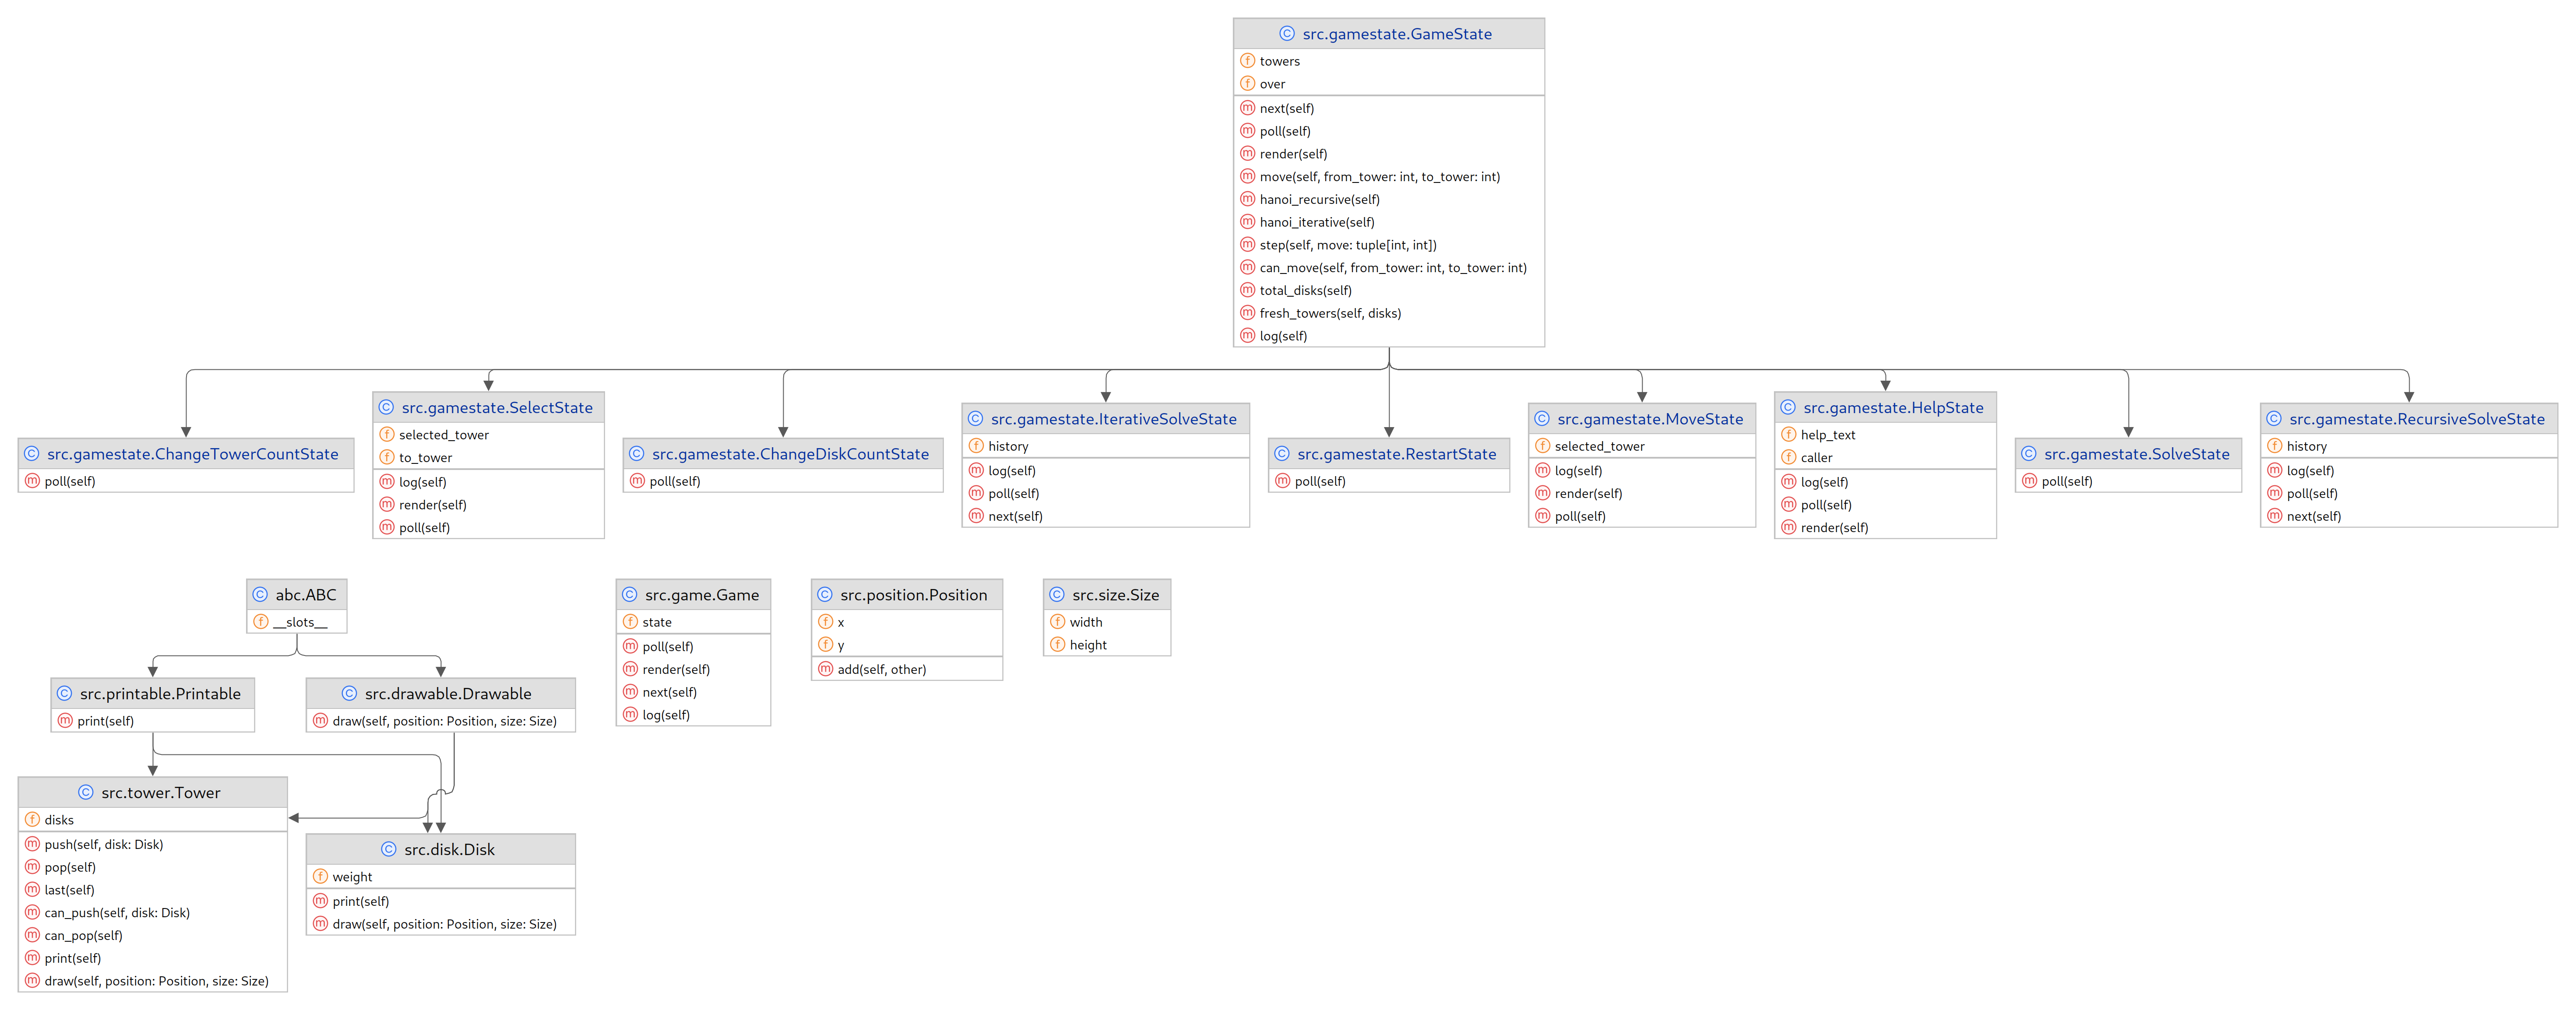
\includegraphics[width=\textwidth]{diagram.png}
		\caption{Диаграмма классов проекта}
	\end{center}
\end{figure}

Как и любая игра нашему проекту нужна инициализация данных (создание
первоначальных башен и дисков в правильном порядке). Инициализация игрового
``движка''. И главный цикл игры, в котором будет происходить в чётком порядке:

\begin{enumerate}
  \item Логирования (log)
  \item Отрисовка (render)
  \item Отслеживание за нажатиями внутри игрового окна (poll)
  \item Изменение состояния игры (next)
\end{enumerate}

Важно отметить, что состоянии игры изменяется не только в методе next, но и,
конечно, вся магия мутации будет происходить внутри poll. Так как игрок будет
нажимать на клавиши клавиатуры, игра будет это воспринимать как собственное
изменение, например, переключение в другой режим игры.

\subsection{Рекурсивный алгоритм на Python}

\begin{code}
	\inputminted[breaklines=true, xleftmargin=1em, linenos, frame=single,
		framesep=10pt, fontsize=\footnotesize, firstline=119,
		lastline=137]{python}{../src/src/gamestate.py}
	\caption{Одна из рекурсивных реализаций алгоритма решения задачи о Ханойской
		башне}
\end{code}


\subsection{Итеративный алгоритм на Python}

\begin{code}
	\inputminted[breaklines=true, xleftmargin=1em, linenos, frame=single,
		framesep=10pt, fontsize=\footnotesize, firstline=139,
		lastline=168]{python}{../src/src/gamestate.py}
	\caption{Одна из итеративных реализаций алгоритма решения задачи о Ханойской
		башне}
\end{code}

\subsection{Тестирование библиотеки}

В ходе выполнения работы были написаны юнит тесты для библиотеки классов.
Было протестировано перемещение дисков между башнями: нельзя допустить, чтобы
диск был помещён не по-правилам пазла.

\section*{Заключение}
Реализовали полноценную игру, рекурсивный и итеративные алгоритмы решения
задачи о Ханойской башне.
\addcontentsline{toc}{section}{Заключение}
